\section{Overview}

\subsection{Machine Learning}
Machine learning is the field of study that focuses on training machines (e.g., computers) to identify patterns and derive logical conclusions \autocite{machDef}. It is technically an imitation of the human learning process and can be divided into two different main types, supervised and unsupervised learning. \\
Supervised learning is used to classify instances to already known categories based on their characteristics. Algorithms that belong to this type are first trained on an already labeled with the possible categories dataset and, afterward, use their gained knowledge to classify new unlabeled datasets \autocite[24]{han}. For example, a supervised learning problem would be images, each one containing one hand-written digit, and its label the number to which it corresponds. After training the algorithm with a labeled set, the algorithm would be capable of recognizing digits on images. \\
Unsupervised learning, on the other side, is used to group data without knowing the labels beforehand and without any training proceeding. This type of learning allows the model to learn by itself. Usually, a person with knowledge in the sector is needed to interpret and extract the knowledge from the created groups \autocite[25]{han}. The above example using unsupervised learning would be giving as input the images to the algorithm without labeling the digits. The expected output would be ten clusters, each one corresponding to one of the digits from zero to nine. A person inspecting the results would be in the position to recognize which is the digit shown on the images of each cluster. \\
Apart from those two main categories, two additional categories are worth mentioning, semi-supervised learning, and reinforcement learning. \\
Semi-supervised learning falls between the above two types. It consists of a small amount of labeled data and a large amount of unlabeled data. The labeled data serve as initial training, and the results are using the unlabeled data to improve the process and, on many occasions, spot outliers \autocite[25]{han}. Using the digits example, let us suppose that labeling all the pictures would be a very costly procedure, therefore someone would label a small amount of the images to use as the training set, and afterward apply the algorithm to the rest of the images to improve the model.
Reinforcement learning is a more interactive method, as opposed to the previous ones. It uses unlabeled data and requires rewards or penalties based on its behavior. This type of machine learning takes decisions that lead to the maximization of the reward taken (e.g., a numerical value) \autocite[2-3]{rein}. Therefore, the digits paradigm would be similar to the one of unsupervised learning, but instead of trying to discover hidden patterns, it would try to find the output with the maximized reward (or minimized penalty). 

\begin{figure}
	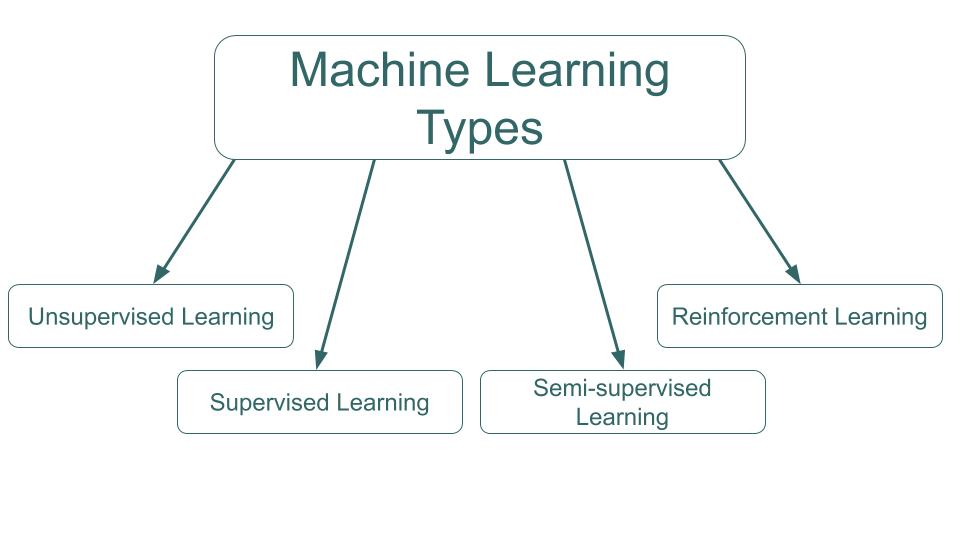
\includegraphics[width=\textwidth]{mach_learn_types}
	\caption{Types of machine learning.}
  	\label{fig:types}
\end{figure}

\subsection{Clustering}
Clustering or cluster analysis is a type of unsupervised machine learning. It groups instances to create coherent sets based on their similarities and dissimilarities. The aim is that instances that belong to the same sets are as much alike and as much different from the instances of the other sets as possible \autocite{dunham, tanSteinKum}. \\
As \textcite{kantar} claims, humans are capable of detecting natural clusters from given data and compete with the clusters created by algorithms up until three-dimensional data. In real life, though, the dimensionality of the data examined is usually much higher than that, and therefore, if the cluster analysis were possible to be done by a human, it would not be as efficient \autocite[250]{kantar}. Since it is not humans that perform clustering, but algorithms, unexpected groups, and patterns can be discovered \autocite[444]{han}.

\subsection{Types of Clustering}
Clustering algorithms can be categorized based on two criterions. The first one is the relationships between the produced clusters of one iteration with the ones of a previous iteration. The second one is the number of clusters an instance can be a part of. \\
Based on the first criterion, \textcite{tanSteinKum} describe the following types: \\
Partitional clustering is a type of clustering which allows no overlapping between two or more sets of clusters, hence partitions the initial set to independent sets. This means that each instance can be part of exactly one cluster. \\
Hierarchical clustering produces clusters in each iteration, which are subsets of a cluster of the previous iteration. This can occur by starting from one cluster, which contains all instances, and repeatedly partition the available clusters to even smaller ones. \\
\textcite{tanSteinKum} mention three more types of clustering in their book, which are formed based on the second criterion and are the following: \\
Exclusive clustering signifies that an instance can only be a part of only one cluster. \\
Overlapping or non-exclusive clustering signifies that an instance can be part of more than one cluster. \\
Fuzzy clustering signifies that every instance belongs to all the clusters \autocite{tanSteinKum}.

\section{K-means}
K-means is a prototype-based, iterative algorithm in which instances are assigned to a cluster in each iteration. The basic algorithm requires as input K points, called centroids, where K is the number of the desired clusters. To define the cluster that one instance belongs to, the algorithm calculates its distance from all the centroids and assigns it to the closest one. Finally, using the produced clusters calculates the new centroids and repeats until it reaches the desired set. To calculate the distances and the new centroids, the cluster mean needs to be defined and calculated \autocite{dunham, tanSteinKum}. \\
In the simple case where there is only one numerical value describing each instance the cluster mean can use the basic mean definition from statistics as follows: \\


\section{Principal Component Analysis (PCA)}


\section{Applications in the touristic sector}
\subsection{Benefit Segmentation}
As \textcite{data-drivenSegmentation} states, companies all around the globe use market segmentation to target their audiences more effectively and consume their resources more efficiently. Cluster analysis is a useful tool for the creation of those segments to create groups of people that seek similar benefits from their travel experiences. These groups not only help in the formation of marketing strategies but also to products that offer higher fulfillment to their consumers \autocite[17]{data-drivenSegmentation}. This type of segmentation was introduced by \textcite{Haley} in 1968 and is called benefit segmentation. The need for the creation of a new way of grouping target groups arose from the fact that tourists' behavior is mainly determined by the benefits they seek to satisfy and not by descriptive factors \autocite[31]{Haley}. \\
A sample application of benefit segmentation using cluster analysis describe \textcite{finland} in their article. Data about tourists were gathered in the region of Savonlinna, Finland, during the period with the highest footfall of the year through electronic questionnaires. The research aims to find the different segments of tourists based on the benefits they seek and then examine the interest of each segment on wellness holidays. \\
For the segment formulation, they used two algorithms, one hierarchical to find the best number of clusters, and K-means to create the clusters. The solution they proposed contained four distinct clusters. From the four clusters, two of them seemed to have a higher preference for wellness services, as designated by \textcite{finland} 'Culturals' and 'Sightseers'. Both clusters portrayed people that seem to favor attractions and also have a tendency to go back to the same destination for their vacation. Additionally, the 'Culturals' show a preference for cultural activities, where 'Sightseers' show a preference for sightseeing activities. The illustrated interpretation of the results is that the previous approach, which promoted wellbeing products based on nature, might not be the most appropriate. The suggested alternative claims that combining wellbeing with history, culture, diverse experiences, and attractions could be more efficient \autocite[308-312]{finland}. \\
Another sample application that focuses more on the nature of the data to be analyzed describes \textcite{categorical}. Commonly, collected touristic data come from surveys, which, to a great extent, contain qualitative data. Furthermore, for the market segmentation to produce more representative results, many attributes should be used. Even so, most clustering methods used by marketers do not work well nor with multidimensional nor with categorical data \autocite[391]{categorical}. \\
\textcite{categorical} used a Bed and Breakfast (B\&B) survey in order to illustrate a more reliable way to deal with this type of data. First, they used multiple correspondence analysis (MCA) to produce some initial cluster groups, get a visualization of them, and understand them. Afterward, they performed cluster analysis, using the k-means algorithm, in order to find the market segments. They concluded in four clusters, from which the three of them seemed to be worthy of further analysis. The other cluster did not contain enough data to lead to meaningful interpretation. The first of the three segments contained respondents who were seeking a romantic experience and were less likely to return to the B\&B. Also, they were not very concerned about the cost and amenities provided. Tourists of the second cluster were looking for cozier, more peaceful, nature-related options and were more likely to go back to the same place if they liked it. They also preferred to take part in energetic activities and, similarly to the first cluster, do not care so much about price and amenities. The third cluster was technically a mixture of the two previous ones. The distinguishing factor was the eagerness of the people of the latter to socialize and the importance of price, value factors \autocite[394-395]{categorical}. \\
Taking into consideration the results of the k-means \textcite{categorical} used the geographical characteristics of each cluster and suggested the usage of different marketing approaches on each of the three regions that the respondents came from (Wisconsin, Minnesota, Illinois). The B\&B owners made some changes based on the formed clusters to improve their customer satisfaction. For example, they decided to offer a private breakfast to the first cluster, add more activities to please the second cluster, and provide information about social events to the people of the last cluster. Furthermore, they were planning on changing their marketing strategy based on the demographics provided by the research to better target their audience \autocite[395-396]{categorical}.